\documentclass[12pt, a4paper]{article}
\usepackage{import}

\usepackage{graphicx}
\usepackage{amssymb}
\usepackage{mathtools}  
\usepackage{amsthm}  
\usepackage{graphicx}
\usepackage{float}
\usepackage{caption}
\usepackage{enumerate}

\import{../../../lib/}{bridge.sty}
\setmainlanguage{english}

\title{Jak radzić sobie z wejściami na 1\nt?}
\author{Krystyna Gasińska}
\begin{document}
\maketitle

\begin{formal}
Uwaga! Pełen system znajduje sie na końcu pliku, ale nie ma sensu uczyć się go na pamięć!
Są tam też wejścia na 1\nt przeciwnika, w ramach powtórki.
\end{formal}

% \section{Naturalne wejścia przeciwnika}
% Zajmiemy się najpierw wejściami, które pokazują naturalny kolor. Uznajemy, że odzywka
% pokazująca kolor tej odzywki (nawet jeśli pokazuje również inny kolor), jest naturalna.
% Na przykład:

% 1\nt\ -- (\alrts{2\hearts}) -- ...\\
% 2\hearts = 5\hearts\ + 4\minor

% jest naturalnym wejściem, bo pokazuje kiery.

Jak radzić sobie z wejściami na nasze (partnera) 1\nt?\\
Podstawowe ustalenie to: po kontrze przeciwnika
gramy normalnie (nadal 2\clubs to Stayman, 
2\diams to transfer na kiery itd.). Tak samo po
wejściu 2\clubs, wtedy \dbl to Stayman, a reszta bez zmian.
Po innych wejściach natomiast: kolory na poziomie 2
są do pasa, kolory na poziomie 3 to \gf. Kontra, jeśli
przeciwnik pokazuje naturalny kolor, jest negatywna.

Ma to oczywiste wady:

\vspace{0.3cm}
\noindent
1.\\
1\nt\ -- (2\spades) -- ?\\
Trzymamy:\\
\chandp{J4}{K97432}{QJ75}{72}{7 \hcp}\\
Chcemy walczyć na poziomie 3, wiemy nawet o ficie, ale 3\hearts to już \gf.

\vspace{0.3cm}
\noindent
2.\\
1\nt\ -- (2\spades) -- ?\\
Trzymamy:\\
\chandp{642}{QT4}{AJ75}{A32}{11 \hcp}\\
Mamy bilans na końcówkę, ale nie mamy koloru do pokazania.
Wrzucamy 3\nt bez trzymania czy \dbl z trzema kierami?

\vspace{0.3cm}
\noindent
3.\\
1\nt\ -- (2\hearts) -- ?\\
Trzymamy:\\
\chandp{AJT43}{K3}{T943}{32}{8 \hcp}\\
Nie wiemy, czy odpowiedni dla nas kontrakt to
4\spades -- jeśli trafimy na fit, 3\nt -- jeśli mamy bilans, ale nie fit, czy może jedynie 2\spades,
jeśli partner ma brzydkie 15\hcp bez fitu. Chcielibyśmy pokazać piki i zainwitować, 
a możemy wybrać tylko między słabym 2\spades i \gf 3\spades.

\vspace{0.5cm}
\noindent
Rozwiązaniem jest 
\textbf{{\color{red}L}{\color{orange}e}{\color{LimeGreen}b}{\color{cyan}e}{\color{blue}n}{\color{purple}s}{\color{red}o}{\color{orange}h}{\color{LimeGreen}l}}:


Po wejściu przeciwnika nie jest nam potrzebne naturalne 2\nt. Bardzo rzadko będzie to 
sam w sobie dobry kontrakt. Dlatego możemy wykorzystać tę odzywkę na coś innego.
2\nt to Lebensohl, na który partner odpowiada automatyczne 3\clubs. Następnie możemy zalicytować
jeszcze raz, np. 3\hearts. Jesteśmy w tej pozycji:

    1\nt\ -- (2\spades) -- 2\nt -- (\pass)\\
    3\clubs -- (\pass) -- 3\hearts

Zauważmy, że pozwoliło nam to zalicytować 3\hearts na dwa sposoby, możemy to zrobić bezpośrednio
po 2\spades,
albo ,,przechodząc przez Lebensohla'' (tak jak powyżej). Dzięki temu możemy odróżnić ręce słabe,
które chcą jedynie przepchać się na poziom 3, od rąk silnych, które chcą sforsować do końcówki.
Umawiamy się, że przejście przez Lebensohla pokazuje rękę słabą, czyli nasze 3\hearts w powyższej licytacji
jest do pasa, a bezpośrednie 3\hearts to \gf.

Rozwiązuje to nasz problem z ręką:\\
\chandp{J4}{K97432}{QJ75}{72}{7 \hcp}\\
Licytacja może przebiegać następująco:

1\nt\ -- (2\spades) -- 2\nt -- (\pass)\\
3\clubs -- (\pass) -- 3\hearts -- all \pass

Analogicznie, zalicytowanie 3\diams po 3\clubs partnera jest słabe (do pasa).
Zauważmy, że jeśli mamy słabą rękę z \textbf{treflami}, możemy po prostu spasować na 3\clubs.

Co w takim razie będzie oznaczało zalicytowanie 3\nt\ ,,przechodząc przez Lebensohla``?
Musi to być oczywiście \gf, gdyż jesteśmy już na poziomie końcówki. Możemy zatem rozróżnić ręce
z trzymaniem i bez trzymania. Umawiamy się, że bezpośrednie 3\nt pokazuje \textbf{brak trzymania},
natomiast 3\nt\ ,,przez Lebensohla`` oznacza: chcę grać 3\nt i mam trzymanie. Jest to zasada 
\textbf{slow shows} (licytowanie \textbf{powoli}, czyli przez Lebensohla \textbf{pokazuje} trzymanie).

Uwaga! Mając to ustalenie trzeba przytomnie licytować:\\
1\nt\ -- (2\spades) -- 3\nt\\
Oznacza brak trzymania i obie osoby w parze muszą o tym pamiętać!

Rozwiązuje to nasz drugi problem. Trzymając:\\
\chandp{642}{QT4}{AJ75}{A32}{11 \hcp}\\
Po wejściu przeciwnika 2\spades możemy po prostu bezpośrednio zalicytować 3\nt. 
Partner, jeśli również nie ma trzymania, postara się znaleźć znaleźć lepszy kontrakt.

A co jeżeli mamy możliwość pokazania koloru na 3 sposoby? Np. po licytacji:

1\nt\ -- (2\hearts) -- ?

Mając piki, możemy je teraz pokazać licytując 2\spades, 3\spades, lub 3\spades przez Lebensohla.
Nie ma oczywiście sensu, żeby 3\spades przez Lebensohla było słabe. Mamy już 2\spades, które 
jest słabe. Logiczne jest zatem, żeby 3\spades przez Lebensohla było \textbf{inwitem}. 

Super! Rozwiązuje to nasz trzeci problem. Trzymając:\\
\chandp{AKJ43}{43}{T943}{32}{8 \hcp}\\
Po otwarciu naszego partnera 1\nt i wejściu przeciwnika 2\hearts, mamy możliwość inwitu:

1\nt\ -- (2\hearts) -- 2\nt -- (\pass)\\
3\clubs -- (\pass) -- 3\spades

Partner może teraz spasować na 3\spades lub przyjąć inwit w 3\nt lub 4\spades, w zależności
od fitu.

Lebensohl działa również, jeśli wejście przeciwnika nie jest naturalne, np. 2\diams = multi.
Ustalenia są dokładnie takie same: kolory na poziomie 2 do pasa, na poziomie 3 \gf,
a przez Lebensohla? Wtedy zależy czego nam brakuje, na przykład:

1\nt\ -- (\alrts{2\diams}) -- 2\nt -- (\pass)\\
3\clubs -- (\pass) -- 3\diams

jest \textbf{słabe}, bo nie mieliśmy możliwości pokazania kar na poziomie 2, ale już:

1\nt\ -- (\alrts{2\diams}) -- 2\nt -- (\pass)\\
3\clubs -- (\pass) -- 3\hearts

jest inwitem z kierami, bo rękę słabą z kierami mogliśmy sprzedać przez bezpośrednie 2\hearts.

Nie zmienia się również ustalenie: 3\nt przez Lebensohla pokazuje trzymanie, bezpośrednie: jego brak.

\begin{formal}
    Niezależnie, czy gramy Lebensohlem, czy przedstawionym
    za chwilę Transfer Lebensohlem, Texas, czyli transfery
    4\diams i 4\hearts pozostają niezmienne w każdej sekwencji.
\end{formal}

\begin{formal}
    Kontra na naturalnie licytowany kolor przeciwnika, jest zawsze \textbf{negatywna}.
    Tzn. wejście 2\clubs = \major nie jest naturalne (bo nie pokazuje trefli),
    ale 2\spades = 5\spades\ + 4\minor uznajemy tu za naturalne,
    bo pokazuje piki.
\end{formal}

Czy rozwiązało to wszystkie możliwe problemy? Nie, ale większość. Powyższy system
będzie dla wielu wystaczający i nie namawiam do czytania dalej. Jeśli nie graliliście do tej pory
Lebensohlem, to wprowadzenie go do systemu jest i tak dużym usprawnieniem. Jeśli jednak od dawna 
nim gracie, można zastanowić się nad wprowadzeniem konwencji przedstawionej poniżej, która, choć może
wydawać się skomplikowana, jest bardzo logiczna. Polecam jednak
zobaczyć sekcje o \textbf{pałowaniu} sztucznych wejść 2\clubs, 2\diams i 2\nt (pod koniec).

\vspace{0.4cm}
\hrule

A zatem, jakie mamy teraz problemy? Jeden rzuca się w oczy: znaleźliśmy możliwość inwitu, jeśli
nasz kolor jest wyższy niż kolor wejścia przeciwnika, czyli np. możemy inwitować z pikami, jeśli
przeciwnik wszedł 2\hearts. Jeśli jednak nasz kolor jest niższy, nie mamy takiej możliwości.

\vspace{0.3cm}
\noindent
4.\\
1\nt\ -- (2\spades) -- ?\\
Trzymamy:\\
\chandp{K3}{AJT43}{T943}{32}{8 \hcp}\\
Analogicznie jak w problemie 3. nie mamy możliwości inwitu. Tym razem Lebensohl go nie rozwiązuje,
bo mamy pecha i nasz kolor jest niższy niż kolor wejścia przeciwnika.

\vspace{0.3cm}
\noindent
5.\\
1\nt\ -- (2\hearts) -- ?\\
Trzymamy:\\
\chandp{543}{A3}{KJT754}{32}{8 \hcp}\\
Mamy ładne źródło lew, 3\nt może być dobrym kontraktem, ale to zależy jak rozłożone
są punkty naszego partnera. Kara możemy pokazać tylko słabe lub \gf.

6. Drugi problem, nieco bardziej subtelny, czyli dlaczego straciliśmy gwiazdkę!?

\begin{figure}[H]
    \centering
    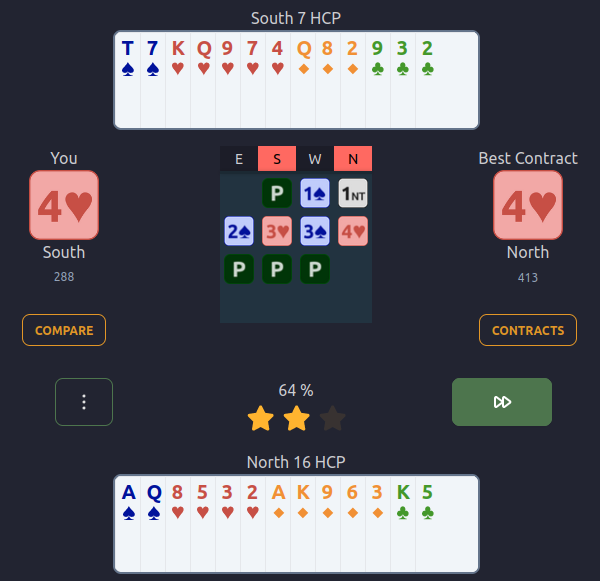
\includegraphics[width=0.7\linewidth]{cuebids.png}
\end{figure}

Partner (na S) nie miał możliwości inwitu, więc zdecydował się na \gf, ale trafił w
16\hcp i 4-kartowy fit. 4\hearts to dobry kontrakt. Czemu straciliśmy gwiazdkę? Gramy ze złej ręki.
Tutaj warto zatrzymać się na chwilę, i odpowiedzieć sobie na pytanie, czemu właściwie
zależy nam na grze z dobrej ręki. Głównym powodem grania transferami po 1\nt nie jest granie z dobrej ręki,
tylko to, żeby osoba znająca bilans rozdania, miała możliwość decydowania o jego wysokości.
Granie z silniejszej ręki zwykle nie jest \textit{aż tak} ważne. Sytuacja zmienia się, gdy mamy do czynienia
z wejściem na 1\nt. Dlaczego? Bo przeciwnicy dokładnie wiedzą w co zawistować. Wist nie tylko
zostanie zagrany \textit{przez} silną rękę w dziadku, ale zostanie zagrany dokładnie w kolor drugiego
przeciwnika, wskazany wejściem. Dlatego przydałoby się, jeśli zdecydujemy się na grę w kolor, 
żeby został on zajęty z ręki ,,przed'' wchodzącym przeciwnikiem.

Odpowiedzią na powyższe problemy jest 
\textbf{{\color{red}R}{\color{orange}u}{\color{LimeGreen}b}{\color{cyan}e}{\color{blue}n}{\color{purple}s}{\color{red}o}{\color{orange}h}{\color{LimeGreen}l}} (aka Transfer Lebensohl).

Sam Lebensohl (2\nt) zostaje bez zmian. Wciąż słabą rękę możemy pokazać licytując najpierw 2\nt.
Zagramy tu co prawda ze złej ręki -- ale nie można mieć wszystkiego.

Co się zatem zmienia? Zamiast licytować kolory na na poziomie 3 naturalnie, licytujemy je transferowo.
A zatem:

1\nt\ -- (2\spades) -- \alrts{3\diams} -- ...

3\diams to transfer na kiery (z piątki). Ponieważ będziemy mieli jeszcze możliwość odezwania się,
siła odzywki 3\diams to \textbf{inwit+}. Możemy mieć siłę jedynie inwitu, lub silną rękę na \gf.
Widać już, że rozwiązuje to problem  z przykładów 4 i 5. Mamy możliwość inwitu, nawet jeśli nasz kolor jest
młodszy, niż kolor wejścia. Rozwiązuje to też problem  z przykładu 6: teraz, jeśli finalnie
znajdziemy się w kontrakcie 3\hearts lub 4\hearts, będziemy grać z dobrej ręki.

Jak odpowiadamy na transfer? Po pierwsze odpowiadamy sobie na pytanie \textbf{czy przyjmujemy inwit}.
Nasz partner może mieć siłę ,,jedynie'' inwitu, więc jeśli nie jesteśmy dość silni, by go przyjąć,
nie możemy odpowiedzieć 3\nt, nawet jeśli nie mamy fitu. Zatem \textbf{przyjęcie transferu oznacza
nieprzyjęcie inwitu}. Nie mówi nic o ficie. Jeśli partner ma silniejszą rękę, będzie miał jeszcze
możliwość zalicytowania.

Na przykład licytacja:

1\nt\ -- (2\spades) -- 3\diams -- (\pass)\\
3\hearts -- all \pass

oznacza, że: licytując 3\diams mieliśmy siłę jedynie na inwit (ponieważ spasowaliśmy na 3\hearts),
a nasz partner nie przyjął inwitu. Nie wiemy czy mamy fit.

Natomiast:

1\nt\ -- (2\spades) -- 3\diams -- (\pass)\\
3\hearts -- (\pass) -- 3\nt -- (\pass)\\
4\hearts -- all \pass

oznacza, że nasz partner nie miał na przyjęcie inwitu, ale my, licytując 3\diams, mieliśmy tak na prawdę
silniejszą rękę. Daliśmy partnerowi możliwość wyboru kontraktu (3\nt), a partner z fitem dla naszych
kierów zdecydował się na 4\hearts.

Jak zatem przyjąć inwit? Jeśli chcemy przyjąć inwit, możemy teraz zastanowić się nad kontraktem.
Zwykle, (w przypadku transferu na kiery), będzie to 3\nt -- jeśli nie mamy fitu, lub 4\hearts, jeśli go mamy.

1\nt\ -- (2\spades) -- 3\diams -- (\pass)\\
4\hearts -- all \pass

Licytacja oznacza: mamy 5 kierów i siłę co najmniej inwitu. Partner ma fit dla naszych kierów i
przyjmuje inwit. Możliwe, że mieliśmy więcej niż inwit, ale nie chcemy licytować dalej (np 10\hcp).

Po wejściu 2\spades mamy zatem:
\begin{itemize}
    \item 2\nt Lebensohl (forsuje 3\clubs)
    \item 3\clubs = transfer na karo, inwit+
    \item 3\diams = transfer na kiery, inwit+
    \item 3\nt = \gf \textbf{bez trzymania}
\end{itemize}

No dobrze, a co z treflami? Pozostają, jak zwykle,
zaniedbane. W przypadku słabej reki z treflami możemy
osiągnąć kontrakt 3\clubs przez Lebensohla (licytujemy
2\nt i pasujemy na 3\clubs partnera), ale nie mamy (i nie będziemy mieć) możliwości
inwitu. \gf na treflach możemy pokazać licytując \textbf{kolor przeciwnika przez Lebensohla}, czyli np.:

1\nt\ -- (2\spades) -- 2\nt -- (\pass)\\
3\clubs -- (\pass) -- 3\spades -- ...

Uwaga! Po wejściu 2\hearts, transfer na piki to 3\diams! Transfer na kiery nie ma sensu,
a dzięki temu, partner, przyjmując inwit ale nie mając fitu ani trzymania, może zalicytować 3\hearts:

1\nt\ -- (2\hearts) -- 2\nt -- (\pass)\\
3\clubs -- (\pass) -- 3\diams -- (\pass)\\
3\hearts -- ...

Jeśli partner nie przyjmuje inwitu, zalicytuje 3\spades:

1\nt\ -- (2\hearts) -- 2\nt -- (\pass)\\
3\clubs -- (\pass) -- 3\diams -- (\pass)\\
3\spades -- ...

System zmienia się nieco po wejściu sztucznym 2\clubs,
pokazującym kolory stare.
2\diams i 2\hearts są nadal słabe (do pasa).
Nie ma sensu, żeby 2\nt było Lebensohlem, bo kara możemy
wygodnie pokazać na poziomie 2, zatem będzie to transfer na trefle.
Zrzekamy się też naturalnego 2\spades, na rzecz
pokazania \textbf{obu młodych} w sile inwit+. 
Zauważmy, że skoro przeciwnik pokazuje stare, to
my często chcemy pokazać młode (a rzadziej naturalne 2\spades).
Jeśli natomiast chcemy grać 2\spades lub 3\clubs, 
możemy wznowić po 2\hearts przeciwników!\\
Kolory na poziomie 3 to nadal Rubensohl, czyli transfery
w sile inwit+ (również na kolor stary!).

\subsubsection*{1\ntx\ -- (\alrts{2\clubs}) -- ?}
2\clubs\ = 5/4 \major
\begin{itemize}
    \item \dbl\ = 8+
    \item 2\diams, 2\hearts = do gry
    \item 2\spades = \minor, inwit+
    \item 2\nt\ = transfer na trefle, inwit+
    \item 3\clubs = transfer na kara, inwit+
    \item 3\diams = transfer na kiery, inwit+
    \item 3\hearts = transfer na piki, inwit+
\end{itemize}

Co z wejściami na poziomie 3? Nie mamy już Lebensohla,
mamy jedynie możliwość inwitu lub \gf (no cóż, zostaliśmy
brutalnie zablokowani). A zatem:

1\nt\ -- (3\clubs) -- ?
\begin{itemize}
    \item 3\diams = transfer na kiery, inwit+
    \item 3\hearts = transfer na piki, inwit+
    \item 3\nt = do gry
\end{itemize}

1\nt\ -- (3\diams) -- ?
\begin{itemize}
    \item 3\hearts = transfer na piki, inwit+
    \item 3\spades = transfer na kiery, \gf \imp
    \item 3\nt = do gry
\end{itemize}

3\spades będące transferem na kiery jest z oczywistego powodu już \gf.

\newpage
\textbf{PRZYKŁADY}

1\nt -- (2\spades) -- ?

\begin{enumerate}
    \item
        \chandp{95}{KT984}{KJ64}{43}{7 \hcp}\\
        Wystarczająco, żeby zawalczyć do 3\hearts.
        Licytujemy 2\nt, a następnie, po odpowiedzi 3\clubs partnera, 3\hearts (do pasa).
    \item
        \chandp{9}{KJT763}{542}{653}{4 \hcp}\\
        Jedynie 4\hcp. Czy chcemy walczyć na poziomie 3? Oczywiście!
        Mamy pewny fit i singla w kolorze przeciwnika.
        Licytujemy 2\nt, a następnie, po odpowiedzi 3\clubs partnera, 3\hearts (do pasa).
    \item 
        \chandp{93}{KQT76}{K42}{653}{8 \hcp}\\
        Chcemy zainwitować. Licytujemy 3\diams.
    \item 
        \chandp{A93}{KQT76}{K42}{53}{12 \hcp}\\
        Chcemy grać końcówkę. Zaczynamy od 3\diams.
    \item 
        \chandp{3}{AKJT76}{Q42}{753}{10 \hcp}\\
        Chcemy grać 4\hearts. Licytujemy 4\diams (Texas).
    \item 
        \chandp{AK}{JT7}{K642}{7653}{11 \hcp}\\
        Chcemy grać 3\nt. Licytujemy je przez Lebensohla -- mamy trzymanie!
        Najpierw 2\nt, a po odpowiedzi 3\clubs partnera, 3\nt.
    \item 
        \chandp{83}{QT7}{KQ42}{A653}{11 \hcp}\\
        Mamy bilans na końcówkę, ale boimy się o trzymanie.
        Nie mamy koloru do pokazania transferem. Licytujemy bezpośrednie 3\nt.
    \item
        \chandp{3}{JT75}{QT92}{A652}{7 \hcp}\\
        Właśnie dlatego \dbl jest negatywna a nie karna.
        Chcemy się przepchać na poziom 3, ale nie
        mamy własnego koloru. Licytujemy: \dbl.
    \item 
        \chandp{AQ32}{5}{QT92}{T652}{8 \hcp}\\
        Tu z kolei przydałaby się kontra karna, albo
        naturalny inwit do 3\nt. Zrzekliśmy się jednak ich,
        na korzyść konwencji, które przynoszą więcej zysków.
        Licytujemy: \pass.
\end{enumerate}

\newpage

1\nt -- (2\spades) -- 3\diams -- (\pass)\\
?

\begin{enumerate}
    \item
        \chandp{KJ7}{Q4}{AQ54}{QJ52}{15 \hcp}\\
        Mamy minimum otwarcia, nie chcemy przyjąć inwitu. 
        Nie mamy fitu, ale nie przyjmując inwitu musimy 
        odpowiedzieć 3\hearts. Jeśli partner ma więcej,
        niż tylko inwit, nie spasuje na 3\hearts.
    \item
        \chandp{K74}{Q4}{AQT}{KQJ2}{17 \hcp}\\
        Chcemy przyjąć inwit. Nie mamy fitu. Licytujemy 3\nt.
    \item
        \chandp{K87}{AQ7}{74}{AK532}{16 \hcp}\\
        Chcemy przyjąć inwit i mamy fit. Licytujemy 
        4\hearts i cieszymy się, że gramy z naszej ręki.
    \item
        \chandp{43}{K4}{AQJ5}{AK52}{17 \hcp}\\
        Chcemy przyjąć inwit. Nie mamy fitu, ale nie mamy
        też żadnego trzymania. Możemy zalicytować 3\spades.
        Będzie to przyjęcie inwitu i informacja dla partnera,
        że boimy się o trzymanie.
    \item
        \chandp{43}{AQ53}{AQJ5}{A52}{17 \hcp}\\
        Mamy piękne 17\hcp i 4 kartowy fit. Jesteśmy
        za silni na zwykłe 4\hearts.
        Możemy pokazać bardzo silne przyjęcie (inwitu i kierów)
        licytując 4\clubs (cue bid).
\end{enumerate}

1\nt -- (2\hearts) -- 3\diams -- (\pass)\\
3\hearts -- (\pass) -- ?
\begin{enumerate}
    \item 
        \chandp{94}{KQ653}{K873}{52}{8 \hcp}\\
        Partner odrzucił inwit. Pasujemy.
\end{enumerate}

1\nt -- (2\hearts) -- 3\clubs -- (\pass)\\
3\diams -- (\pass) -- ?
\begin{enumerate}
    \item 
        \chandp{A4}{43}{KQJ763}{752}{10 \hcp}\\
        Mamy na \gf, więc nie chcemy spasować, mimo że
        partner odrzucił ,,inwit''. Nie mamy trzymania, i możemy to pokazać
        licytując 3\hearts.
\end{enumerate}

1\nt -- (2\spades) -- 3\diams -- (\pass)\\
3\spades -- (\pass) -- ?
\begin{enumerate}
    \item 
        \chandp{63}{AJ763}{KQJ7}{75}{11 \hcp}\\
        Partner pokazał przyjęcie ,,inwitu'', ale brak fitu i
        obawę o trzymanie. My też nie mamy trzymania. Szukamy
        innego kontraktu licytując naturalne 4\diams. Możliwe,
        że partner zalicytuje 4\hearts i zagramy na 7-karcie (co jest zwykle
        lepsze niż granie 5\minor!).
\end{enumerate}

\vspace{1cm}
\textbf{WIELKIE PAŁOWANIE}

Na sztuczne wejścia, tj. 2\clubs = \major, 2\nt = \minor i 2\diams = multi,
kontra jest \textbf{karna} i pokazuje 8+\hcp.
Taka kontra oznacza, że jesteśmy \textit{sforsowani do 2\nt}, czyli przeciwnicy
nie mogą grać \textbf{bez kontry} na poziomie 2.

Przykłady:
1\nt -- (\alrts{2\clubs}) -- ?
\begin{enumerate}
    \item 
        \chandp{A63}{K63}{732}{KJ73}{11 \hcp}\\
        Mamy 11\hcp. Owszem, możemy grać 3\nt, ale może bardziej opłaca się spałować przeciwników?
        W końcu mają maksymalnie 14\hcp na linii i mogą nie mieć fitu!
        Licytujemy \dbl.
    \item 
        \chandp{3}{KJ53}{732}{KQ873}{9 \hcp}\\
        Możliwe, że przeciwnicy znajdą fit pikowy, a nasz partner nie będzie
        mógł ich spałować. Ale jeśli zalicytują kiery, mamy idealną rękę na kontrę.
        Licytujemy \dbl.
\end{enumerate}

1\nt -- (\alrts{2\clubs}) -- \dbl -- (2\hearts)\\
?
\begin{enumerate}
    \item 
        \chandp{AJ3}{KJ63}{73}{AQ73}{15 \hcp}\\
        Pała!
    \item 
        \chandp{AJ32}{J63}{K3}{AQ73}{15 \hcp}\\
        Nie możemy spałować kierów. Ale jeśli nasz partner
        to zrobi, z radością spasujemy na kontrę.
        Mamy pewność, że nasz partner nie spasuje na
        2\hearts -- jego pierwotna kontra nie pozwala nam
        dać przeciwnikom grać 2\hearts.
\end{enumerate}

1\nt -- (\alrts{2\clubs}) -- \dbl -- (2\hearts)\\
\pass -- (\pass) -- ?
\begin{enumerate}
    \item 
        \chandp{3}{KJ53}{732}{KQ873}{9 \hcp}\\
        Pała!
    \item 
        \chandp{AJ32}{63}{K32}{9873}{8 \hcp}\\
        Nasz partner nie mógł spałować kierów i my też nie mamy na kontrę.
        Teraz chcielibyśmy dać kontrę negatywną, ale kontra jest karna...
        Ale \textbf{nie możemy spasować}! Licytujemy 2\nt
        w poszukiwaniu własnego koloru.
\end{enumerate}

1\nt -- (\alrts{2\clubs}) -- \dbl -- (2\spades)\\
\dbl -- (\pass) -- ?
\begin{enumerate}
    \item 
        \chandp{J32}{KJ63}{73}{AQ73}{11 \hcp}\\
        Nasz partner spałował piki. Możemy spokojnie
        spasować.
    \item
        \chandp{3}{KJ53}{J32}{KQ873}{10 \hcp}\\
        Nasz partner spałował piki, ale mógł to zrobić nawet z trzecim KJ...
        Nie możemy spasować. Licytujemy 3\nt.
\end{enumerate}

\begin{formal}
Przy pałowaniu przeciwnika ważne są \textbf{założenia}. 
W korzystnych jesteśmy bardziej skłonni do pałowania,
wystarczy, że obłożymy bez 2 i już zarobimy więcej niż za
własną końcówkę! Jeśli jesteśmy w niekorzystnych, to musimy
obłożyć przeciwników bez 4, żeby się opłacało (jeśli idzie nam końcówka).
\end{formal}

\newpage

\textbf{{\color{red}S}{\color{orange}Y}{\color{LimeGreen}S}{\color{cyan}T}{\color{blue}E}{\color{purple}M}}\\

Wejścia na 1\nt przeciwnika:

\subsubsection*{(1\ntx) -- ?}
\begin{itemize}
    \item \dbl\ = 5\minor\ + 4\major
    \item 2\clubs\ = 54 \major
    \item 2\diams\ = 6+ \major
    \item 2\hearts\ = 5\hearts\ + 4\minor
    \item 2\spades\ = 5\spades\ + 4\minor
    \item 2\nt = 55 \minor
\end{itemize}

\subsubsection*{(1\ntx) -- \dbl\ -- (P) -- ?}
\begin{itemize}
    \item 2\clubs\ = \pass/correct
    \item 2\diams\ = show major
    \item 2\hearts/2\spades = own suit
\end{itemize}

\subsubsection*{(1\ntx) -- 2\clubs\ -- (P) -- ?}
\begin{itemize}
    \item 2\diams\ = show better major
    \item 2\hearts, 2\spades\ = preference
\end{itemize}

\subsubsection*{(1\ntx) -- 2\diams\ -- (P) -- ?}
\begin{itemize}
    \item 2\hearts\ = \pass/correct
    \item 2\spades\ = \inv with \hearts
\end{itemize}

Przeciwnik wchodzi na nasze 1\nt:

\subsubsection*{1\ntx\ -- (2\clubs) -- ?}
2\clubs\ = \clubs
\begin{itemize}
    \item \dbl\ = Stayman
\end{itemize}

\textsc{system on}

\subsubsection*{1\ntx\ -- (\alrts{2\clubs}) -- ?}
2\clubs\ = 5/4 \major
\begin{itemize}
    \item \dbl\ = 8+
    \item 2\diams, 2\hearts = to play
    \item 2\spades = \minor, \invp
    \item 2\nt\ = 5+\clubs, \invp
    \item 3\clubs\ = 5+\diams, \invp
    \item 3\diams\ = 5+\hearts, \invp
    \item 3\hearts\ = 5+\spades, \invp
\end{itemize}

\subsubsection*{1\ntx\ -- (2\diams) -- ?}
2\diams\ = \diams
\begin{itemize}
    \item \dbl\ = negative
    \item 2\hearts, 2\spades\ = to play
    \item 2\nt\ = Lebensohl
    \item 3\clubs\ = 5+\hearts, \invp
    \item 3\diams\ = 1-\diams, \invp
    \item 3\hearts\ = 5+\spades, \invp
    \item 3\spades\ = 5+\clubs, \gf
    \item 3\nt\ = no \diams\ stopper
    \item 4\diams, 4\hearts\ = Texas
\end{itemize}

\subsubsection*{1\ntx\ -- (\alrts{2\diams}) -- ?}
2\diams\ = 6+ \major
\begin{itemize}
    \item \dbl\ = 8+
    \item 2\hearts, 2\spades\ = to play
    \item 2\nt\ = Lebensohl
    \item 3\clubs\ = 5+\diams, \invp
    \item 3\diams\ = 5+\hearts, \invp
    \item 3\hearts\ = 5+\spades, \invp
    \item 3\spades\ = 5/5 \minor
    \item 3\nt\ = to play
    \item 4\diams, 4\hearts\ = Texas
\end{itemize}


\subsubsection*{1\ntx\ -- (2\hearts) -- ?}
\begin{itemize}
    \item \dbl\ = negative
    \item 2\spades\ = to play
    \item 2\nt\ = Lebensohl
    \item 3\clubs\ = 5+\diams, \invp
    \item 3\diams\ = 5+\spades, \invp
    \item 3\hearts\ = 1-\hearts, \gf
    \item 3\spades\ = 55 \minor, \gf
    \item 3\nt\ = no \hearts\ stopper
    \item 4\hearts\ = Texas
\end{itemize}

\subsubsection*{1\ntx\ -- (2\spades) -- ?}
\begin{itemize}
    \item \dbl\ = negative
    \item 2\nt\ = Lebensohl
    \item 3\clubs\ = 5+\diams, \invp
    \item 3\diams\ = 5+\hearts, \invp
    \item 3\hearts\ = 55\minor, \gf
    \item 3\spades\ = 1-\spades, \gf
    \item 3\nt\ = no \spades\ stopper
    \item 4\diams\ = Texas
\end{itemize}

\subsubsection*{1\ntx\ -- (\alrts{2\nt}) -- ?}
2\nt\ = \minor
\begin{itemize}
    \item \dbl\ = 10+
    \item 3\clubs\ = Stayman
    \item 3\diams\ = 5+\hearts, \invp
    \item 3\hearts\ = 5+\spades, \invp
\end{itemize}

\subsubsection*{1\ntx\ -- (3\clubs) -- ?}
\begin{itemize}
    \item \dbl\ = negative
    \item 3\diams\ = 5+\hearts, \invp
    \item 3\hearts\ = 5+\spades, \invp
    \item 3\spades\ = 5+\diams, \gf
    \item 3\nt\ = to play
\end{itemize}

\subsubsection*{1\ntx\ -- (3\diams) -- ?}
\begin{itemize}
    \item \dbl\ = negative
    \item 3\hearts\ = 5+\spades, \invp
    \item 3\spades\ = 5+\hearts, \gf
    \item 3\nt\ = to play
\end{itemize}

\subsubsection*{1\ntx\ -- (\dbl) -- ?}

\textsc{system on}

\newpage

Behind the scenes:
\begin{figure}[H]
    
\includegraphics[width=0.4\linewidth]{cuebids2.png}
\end{figure}


\end{document}
